\documentclass{article}
\usepackage{amsmath, amssymb, geometry}
\usepackage{tikz}
\usepackage{titlesec}
\usepackage{graphicx}
\usepackage{caption}
\usepackage{subcaption}
\usepackage{float}
\usepackage{lmodern}
\usepackage[french]{babel}
\usepackage{hyperref}

\newcommand{\HRule}{\rule{\linewidth}{0.5mm}}
\geometry{a4paper, margin=2.5cm}
\date{\vspace{1cm} \today}

\begin{document}

% Page de titre
\begin{titlepage}
    \centering
    \begin{tikzpicture}[remember picture, overlay]
        \node[opacity=0.1] at (current page.center) {
\includegraphics[width=\paperwidth,height=\paperheight,keepaspectratio]{image.png}};
    \end{tikzpicture}

    \vspace*{2cm}

    {\Huge\bfseries Rapport de modélisation\\[0.5em] \LARGE SAE821 -- Gérer un projet}

    \vspace{1.5cm}

    \HRule
    \vspace{0.5cm}

    \Large{Modélisation UML et architecture du projet}

    \vspace{0.5cm}
    \HRule\\[11cm]

    \begin{flushleft}
        \small
        \textbf{Pegliasco Matteo}\\
        \textbf{Berge Enzo}\\
        \textbf{Audouard Florian}\\
        \textbf{Hermelin Lois}\\
        \textbf{Master Informatique et Mathématiques}\\
        Université de Toulon, La Garde, Var, France
    \end{flushleft}
    \vfill
\end{titlepage}

% ===========================
\section{Introduction}
Présentation du projet, du contexte général, et des objectifs poursuivis dans le cadre de la modélisation.

\section{Méthodologie}
Définir les outils (ex. StarUML), langages et normes suivis. Présentation des trois axes de modélisation UML : Fonctionnel, Statique et Dynamique.

% ===========================
\section{Modélisation selon l'Axe Fonctionnel}
\subsection{Diagramme de Cas d’Utilisation}
\begin{figure}[H]
    \centering
    \includegraphics[width=0.8\textwidth]{cas_utilisation.png}
    \caption{Diagramme de cas d’utilisation}
\end{figure}

\subsection{Analyse des Acteurs et Scénarios}
Décrivez ici les rôles des acteurs, leurs interactions, et les cas d'utilisation détaillés.

% ===========================
\section{Modélisation selon l'Axe Statique}
\subsection{Diagramme de Classes}
\begin{figure}[H]
    \centering
    \includegraphics[width=\textwidth]{classes.png}
    \caption{Diagramme de classes}
\end{figure}

\subsection{Structure et Relations des Entités}
Analyse des attributs, méthodes, associations, agrégations, généralisations, etc.

% ===========================
\section{Modélisation selon l'Axe Dynamique}
\subsection{Diagramme de Séquence}
\begin{figure}[H]
    \centering
    \includegraphics[width=0.9\textwidth]{sequence.png}
    \caption{Diagramme de séquence pour un scénario clé}
\end{figure}

\subsection{Diagramme d’États}
\begin{figure}[H]
    \centering
    \includegraphics[width=0.7\textwidth]{etats.png}
    \caption{Diagramme d’états pour un objet du système}
\end{figure}

\subsection{Diagramme d’Activités (optionnel)}
\begin{figure}[H]
    \centering
    \includegraphics[width=0.8\textwidth]{activites.png}
    \caption{Diagramme d’activités}
\end{figure}

% ===========================
\section{Analyse Complémentaire (optionnelle)}
\subsection{Diagramme de Composants}
\begin{figure}[H]
    \centering
    \includegraphics[width=0.75\textwidth]{composants.png}
    \caption{Diagramme de composants (si pertinent)}
\end{figure}

\subsection{Diagramme de Déploiement}
\begin{figure}[H]
    \centering
    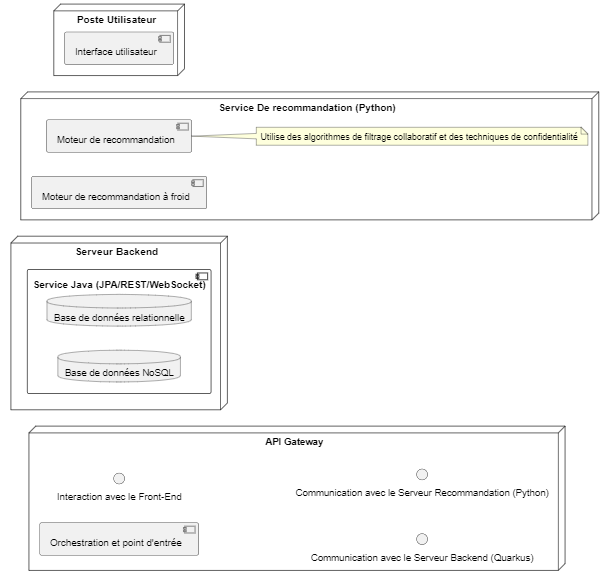
\includegraphics[width=0.75\textwidth]{deploiement.png}
    \caption{Diagramme de déploiement (si pertinent)}
\end{figure}

% ===========================
\section{Conclusion}
\subsection{Bilan de la modélisation}
Synthèse de ce qui a été modélisé, cohérence de l’ensemble, points forts.

\subsection{Perspectives}
Pistes d'amélioration, extensions possibles, outils ou technologies futures.

% ===========================
\appendix
\section{Annexes}
Ajoutez ici :
\begin{itemize}
    \item Les descriptions textuelles complètes des cas d’utilisation
    \item Des diagrammes intermédiaires ou brouillons
    \item Tableaux de correspondance ou d’attribution des tâches
\end{itemize}

\end{document}
